\section[Empirical Determination]{Empirical Determination}

\begin{frame}{Empirical Determination}
	\begin{itemize}
		\item Linear and logistic regressions are simple algorithms with a solid theoretical framework for deriving confidence intervals and prediction regions from \textbf{a single training run}.
		\pause
		\item Unfortunately, this is not the case for all the learning algorithms we will study in this course.
		\pause
		\item In this section, we will see how these intervals and regions can be obtained \textbf{empirically}, and we will compare the empirical results with the theoretical results obtained previously.
		\item We will use the \textbf{bootstrapping} algorithm to generate \textbf{multiple} training instances and thus derive these intervals and regions.
	\end{itemize}
\end{frame}

\begin{frame}{Algorithm Notations}
	\begin{itemize}
		\item We denote the $n$ observations of the training data as $\mathcal{D} = \{(x^{(i)}, y^{(i)})\}_{i=1}^n$.
		\item We denote $\mathcal{D}^{(b)}$ for $b=1, 2, \dots, B$ as the $B$ generated bootstraps.
		\item We denote $\{X_i^{(1)}, X_i^{(2)}, \dots, X_i^{(m)}\}$ as the $m$ input features for inference.
		\item We denote $a: \mathcal{M}_{n,1}(\mathbb{R}) \to \mathbb{R}$ as a function that returns a random element from a column vector $A$ following a uniform distribution: $a(A) = A_j, \, j \sim \mathcal{U}(1, 2, \dots, n)$.
	\end{itemize}
\end{frame}

\begin{frame}[allowframebreaks]{Linear Regression}
	\begin{enumerate}
		\item Calculate $\hat{\beta}$ using all training data $\mathcal{D}$ with the least squares method.
		\item Calculate the residuals on $\mathcal{D}$: $R = Y - \hat{Y}$.
		\item Repeat the following steps for each bootstrap $b$:
		\begin{itemize}
			\item Determine the training data $\mathcal{D}^{(b)}$.
			\item Calculate $\hat{\beta}^{(b)}$ by the least squares method on $\mathcal{D}^{(b)}$.
			\item Calculate $\hat{Y}_i^{(b)}$ from the inference data $X_i$: $\hat{Y}_i^{(b)} = \Phi(X_i) \hat{\beta}^{(b)}$.
		\end{itemize}
		\item For each input $k$ of $X_i$, calculate the $\alpha / 2$ and $1 - \alpha / 2$ quantiles on $\{(\hat{y}_i^{(k)})^{(1)}, (\hat{y}_i^{(k)})^{(2)}, \dots, (\hat{y}_i^{(k)})^{(B)}\}$. This yields the $1 - \alpha$ level confidence interval for $X_i^{(k)}$.
		\item For each bootstrap $b$ and all $X_i$, randomly associate a residual with the predictions: $\left(\hat{y}_i^*\right)^{(b)} = \left(\hat{y}_i\right)^{(b)} + a(R)$.
		\item For each input $k$ of $X_i$, calculate the $\alpha / 2$ and $1 - \alpha / 2$ quantiles on $\{(\hat{y}_i^{*(k)})^{(1)}, (\hat{y}_i^{*(k)})^{(2)}, \dots, (\hat{y}_i^{*(k)})^{(B)}\}$. This yields the $1 - \alpha$ level prediction interval for $X_i^{(k)}$.
	\end{enumerate}
\end{frame}

\begin{frame}{Example: Linear Regression}
	\begin{columns}
		\begin{column}{0.5\textwidth}
			\begin{figure}
				\centering
				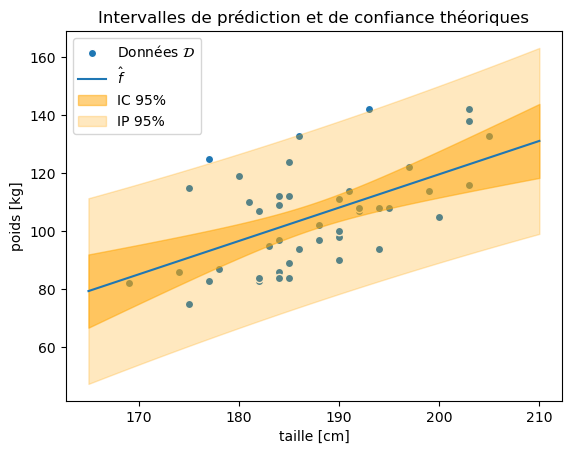
\includegraphics[width=1.0\linewidth]{Images/IP_IC_lineaire_theorie}
				\label{fig:PI_CI_linear_theory}
			\end{figure}
		\end{column}
		\begin{column}{0.5\textwidth}
			\begin{figure}
				\centering
				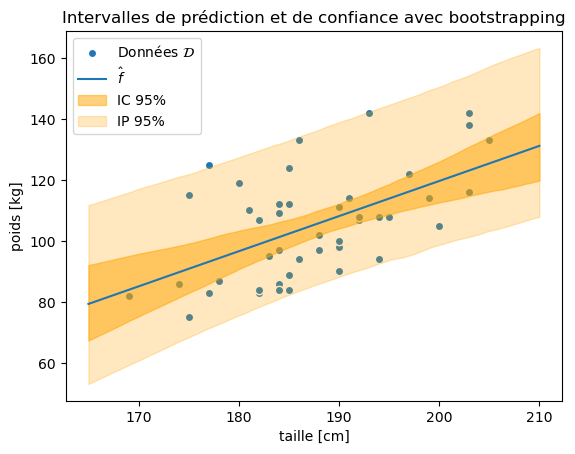
\includegraphics[width=1.0\linewidth]{Images/IP_IC_lineaire_bootstrap}
				\label{fig:PI_CI_linear_bootstrap}
			\end{figure}
		\end{column}
	\end{columns}
	We obtain very similar results using theory and bootstrapping.
\end{frame}

\begin{frame}[allowframebreaks]{Logistic Regression}
	\begin{enumerate}
		\item Calculate $\hat{\beta}$ using all training data $\mathcal{D}$ with the least squares method.
		\item Repeat the following steps for each bootstrap $b$:
		\begin{itemize}
			\item Determine the training data $\mathcal{D}^{(b)}$.
			\item Calculate $\hat{\beta}^{(b)}$ on $\mathcal{D}^{(b)}$ with logistic regression.
			\item Calculate $\hat{p}_i^{(b)}$ from the inference data $X_i$: $\hat{p}_i^{(b)} = \sigma(\Phi(X_i) \hat{\beta}^{(b)})$.
		\end{itemize}
		\item For each input $k$ of $X_i$, calculate the $\alpha / 2$ and $1 - (\alpha / 2)$ quantiles on $\{(\hat{p}_i^{(k)})^{(1)}, (\hat{p}_i^{(k)})^{(2)}, \dots, (\hat{p}_i^{(k)})^{(B)}\}$. This yields the $1 - \alpha$ level confidence interval for $X_i^{(k)}$.
		\item For each input $k$ of $X_i$, the prediction space $C(x_i^{(k)})$ is determined in a manner similar to the theoretical approach:
		\begin{equation}
			C(x_i^{(k)}) = 
			\begin{cases}
				\{0\} & \text{if} \, \hat{p}_{1-\alpha/2}^{(k)} \le \alpha \\
				\{1\} & \text{if} \, \hat{p}_{\alpha/2}^{(k)} \ge 1 - \alpha \\
				\{0, 1\} & \text{otherwise}
			\end{cases}
			\nonumber
		\end{equation}		
	\end{enumerate}
\end{frame}

\begin{frame}{Example: Logistic Regression}
	\begin{columns}
		\begin{column}{0.5\textwidth}
			\begin{figure}
				\centering
				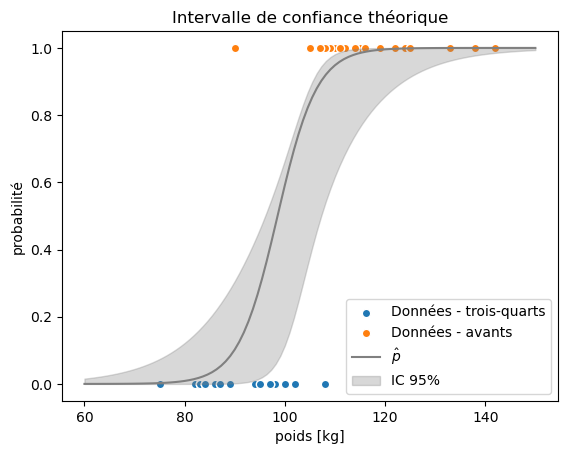
\includegraphics[width=1.0\linewidth]{Images/IP_IC_logistique_theorie}
				\label{fig:PI_CI_logistic_theory}
			\end{figure}
		\end{column}
		\begin{column}{0.5\textwidth}
			\begin{figure}
				\centering
				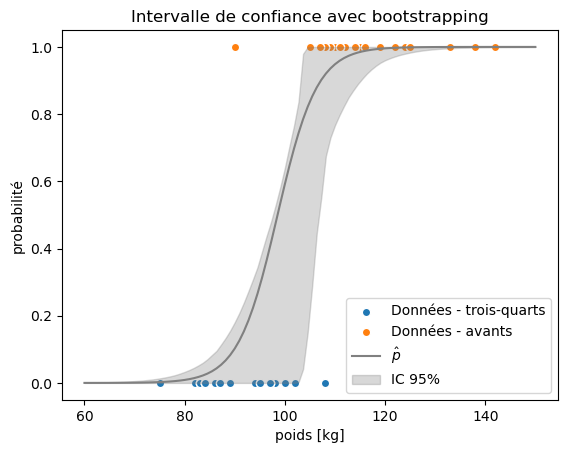
\includegraphics[width=1.0\linewidth]{Images/IP_IC_logistique_bootstrap}
				\label{fig:PI_CI_logistic_bootstrap}
			\end{figure}
		\end{column}
	\end{columns}
	We obtain fairly similar results using theory and bootstrapping.
\end{frame}

\begin{frame}{Example: Logistic Regression}
	\begin{columns}
		\begin{column}{0.5\textwidth}
			\begin{figure}
				\centering
				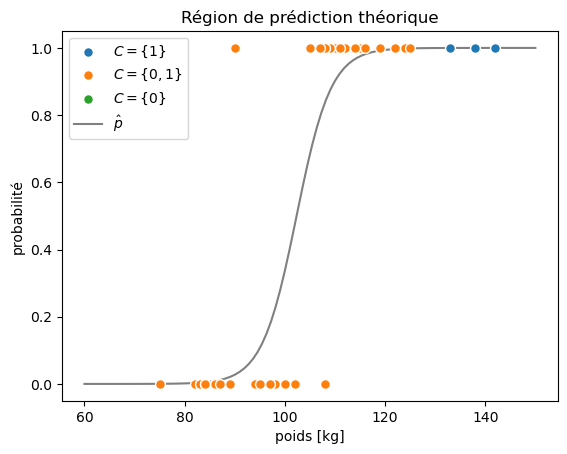
\includegraphics[width=0.95\linewidth]{Images/region_prediction_theorique}
				\label{fig:prediction_region_theory}
			\end{figure}
		\end{column}
		\begin{column}{0.5\textwidth}
			\begin{figure}
				\centering
				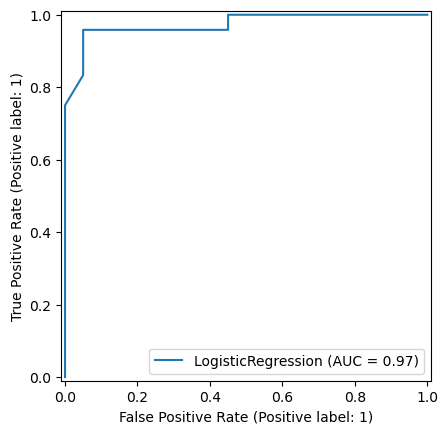
\includegraphics[width=0.85\linewidth]{Images/ROC}
				\label{fig:ROC}
			\end{figure}
		\end{column}
	\end{columns}
	Even if the ROC curve shows that our algorithm captures trends well, the prediction region is much more demanding and only shows a few (5) players confidently classified as forwards. For all other players, logistic regression is much less categorical.
\end{frame}